\documentclass[12pt,a4paper,oneside]{article}
\usepackage[utf8]{inputenc}
\usepackage[czech]{babel}
\usepackage[T1]{fontenc}
\usepackage{amsmath}
\usepackage{amsfonts}
\usepackage{amssymb}
\usepackage{makeidx}
\usepackage{graphicx}
\usepackage{enumerate}
\usepackage[font=small, labelfont=small, labelfont=bf]{caption} %Zobrazení textu "Obr. 3.1:" tučně podle normy; "font=small" písmo podle normy musí být o 2 body menší 
\usepackage[unicode=true]{hyperref} %zobrazení kapitol v pdf rejsříku + hyperaktivnost; unicode=true důležité pro správné zobrazení znaků v pdf rejstříku
\usepackage{indentfirst} %odsazení i prvního odstavce po nadpisu pro lepší strukturu
\usepackage{fancyhdr} %záhlaví a zápatí
\usepackage[left=3.5cm,right=2cm,top=3cm,bottom=3cm]{geometry}
\addto\captionsczech{\renewcommand{\figurename}{Obr.}} %V popisu obrázku zobrazí správně podle normy "Obr." místo "Obrázek"
\addto\captionsczech{\renewcommand{\tablename}{Tab.}} %V popisu tabulky zobrazí správně podle normy "Tab." místo "Tabulka"
\numberwithin{equation}{section} %Přidává k číslu rovnice číslo kapitoly (sekce)
\numberwithin{figure}{section} %Přidává k číslu obrázku číslo kapitoly (sekce)
\numberwithin{table}{section} %Přidává k číslu tabulky číslo kapitoly (sekce)
\frenchspacing %správné dělání mezer
\sloppy %dovoluje Texu dělat větší mezery a odstraňuje problém s přečnívajícími řádky
\setlength{\parindent}{5ex} %správné odsazení na pět úhozů (písmene "x")
\setlength{\parskip}{1ex} %mezera na výšku "x" mezi odstavci pro lepší čitelnost
\author{Lukáš Brtna}
\title{Diplomová práce - HF Modul pro Agros}

\begin{document}
\renewcommand\refname{Použitá literatura} %Místo slova "Reference" u Bibliography
\newcommand{\tg}{\mathop{\rm tg}\nolimits} %Přidává schopnost psát "tg" v rovnici automaticky vpřímeným písmem
\newcommand{\cotg}{\mathop{\rm cotg}\nolimits} %Přidává schopnost psát "cotg" v rovnici automaticky vpřímeným písmem
\newcommand{\grad}{\mathop{\rm grad}\nolimits} %Přidává schopnost psát "grad" v rovnici automaticky vpřímeným písmem
\newcommand{\rot}{\mathop{\rm rot}\nolimits} %Přidává schopnost psát "rot" v rovnici automaticky vpřímeným písmem
\newcommand{\udiv}{\mathop{\rm div}\nolimits} %Přidává schopnost psát "div" v rovnici automaticky vpřímeným písmem; zde se musí použít "\udiv", protože "\div" je již obsazeno systémem
\newcommand{\ud}{\mathrm{d}} %Přidává schopnost psát "d" v rovnici automaticky vpřímeným písmem



%%Začátek úvodní nečíslované sekce%%
\pagestyle{empty} %nečíslování stránek


%%Titulní stránka%%
\begin{titlepage} 
\begin{center}

%%Horní nadpisy%%
\begin{large}
\textbf{ZÁPADOČESKÁ UNIVERZITA V PLZNI\\
~FAKULTA ELEKTROTECHNICKÁ\\
\vspace*{5mm}}
\end{large}
\textbf{~KATEDRA TEORETICKÉ ELEKTROTECHNIKY}
%tex sází křivě - není zarováno přesně na střed - musím cpát mezery na dorovnání
\vspace{70mm}\\

%%Prostřední nadpis%%
\begin{Huge}
\textbf{DIPLOMOVÁ PRÁCE}
\vspace{8mm}\\
\end{Huge}
\begin{LARGE}
Modelování vf zařízení \vspace{90mm}\\
\end{LARGE}
\end{center}

%%Spodní text%%
\begin{flushleft}
\begin{large}
\textbf{Plzeň 2013}
\hfill
\textbf{Lukáš BRTNA}
\end{large}
\end{flushleft}
\end{titlepage}
\newpage


%%Anotace%%
\section*{Anotace}
Účelem diplomové práce je nastínit problematiku vf obvodů a šíření vf vln, 				matematický popis vf šíření a následné zapracování získaných znalostí ve formě 			odvozených slabých forem do xml modulu pro Agros.
\vspace{100mm}\\

%%Klíčová slova%%
\section*{Klíčová slova}
TE vlna, TM vlna, TEM vlna, slabá forma, vf modelování
\newpage


%%Abstract%%
\section*{Abstract}
The objective of the diploma thesis is to summarize hf wave propagation and create 		mathematical description of hf wave propagation. The knowledge is subsequently 			processed in the weak forms of propagation and creation an xml modul for Agros2D.
\vspace{100mm}\\

%%Keywords%%
\section*{Keywords}
TE Wave, TM Wave, TEM Wave, Weak Form, HF Modelling
\newpage


%%Prohlášení%%
\vspace*{50mm}
\section*{Prohlášení}
Předkládám tímto k posouzení a obhajobě diplomovou práci, zpracovanou na závěr 			studia na Fakultě elektrotechnické Západočeské univerzity v Plzni.

Prohlašuji, že jsem tuto diplomovou práci vypracoval samostatně, s použitím odborné 	literatury a pramenů uvedených v seznamu, který je součástí této diplomové práce.
\vspace{\fill}
\begin{flushleft}
V Plzni dne \today
\hspace{\fill}
Jméno a příjmení~~~~~~~~\vspace{3mm}
\end{flushleft}
\begin{flushright}
..............................................
\end{flushright}
\newpage


%%Poděkování%%
\vspace*{50mm}
\section*{Poděkování}
Tímto bych rád poděkoval vedoucímu diplomové práce, panu Ing. Davidu Pánkovi, za 			jeho cenné rady a profesionální vedení bez nějž by vznik této práce nebyl vůbec 			možný.\\
\newpage


%%Definice záhlaví a zápatí
\fancypagestyle{plain}{	%definice záhlaví a zápatí u plain stránek stylu fancy
  \lhead{\textit{Modelování vf zařízení}}
  \rhead{Lukáš Brtna~~~2013}
  \cfoot{- \thepage -}
}
\lhead{\textit{Modelování vf zařízení}}
\rhead{Lukáš Brtna~~~2013}
\cfoot{-~\thepage ~-}
\pagestyle{fancy}
\setcounter{page}{1}


%%Obsah%%
\setlength{\parskip}{0ex} %Aby nebyly moc velké mezery mezi řádky obsahu
\tableofcontents
\newpage


%%Seznam symbolů a zkratek%%
\phantomsection %Pro správné zobrazení čísla stránky v pdf rejsříku a přesný hyperodkaz 
\addcontentsline{toc}{section}{Seznam symbolů a zkratek}
\section*{Seznam symbolů a zkratek}

\begin{tabular}{ll}
\textbf{AFB}\dotfill & Astro-fyzikální Borec \\  
\textbf{NMNS}~\ldots\ldots\ldots & Nejlepší Město Na Světě \\ 
\textbf{MK}\dotfill & Mini-kára \\ 
\end{tabular} 
\newpage

\setlength{\parindent}{5ex} 
\setlength{\parskip}{1ex}


%%Úvod%%
\section{Úvod}
Bylo nebylo. Za sedmero horami a sedmero řekami existoval program jménem Agros2D. Za jeho vývojem stáli udatní bojovníci katedry KTE jako Ing. David Pánek, Ing. Martin Mach nebo Ing. Václav Kotlan, Ph.D. v čele s chrabrým doc. Ing. Pavlem Karbanem, Ph.D. zvaným ,,Filek''. 
\newpage

\section{Šíření vln o vysoké frekvenci}
\subsection{Letí si to světem}
Množství informace I jevu xi ze souboru vzájemně vylučujících se jevů X je kvantifikovatelnou veličinou.

Když se má začít nový odstavec, musí se fyzicky vynechat řádek ve zdrojovém souboru. Nepoužívá se příkaz pro začátek nového řádku. Zajímavé, není-liž pravda?


%%Stránka pro zkoušení vkládání obrázků%%
\newpage
\section{Zatím moje pokusy}
\subsection{Vkládání obrázků}
\begin{figure}[h] %obrázek musí být v plovoucím objektu figure; pro zabránění nežádoucího plavání po stránce se musí doplnit parametr "[h]"
\begin{center}
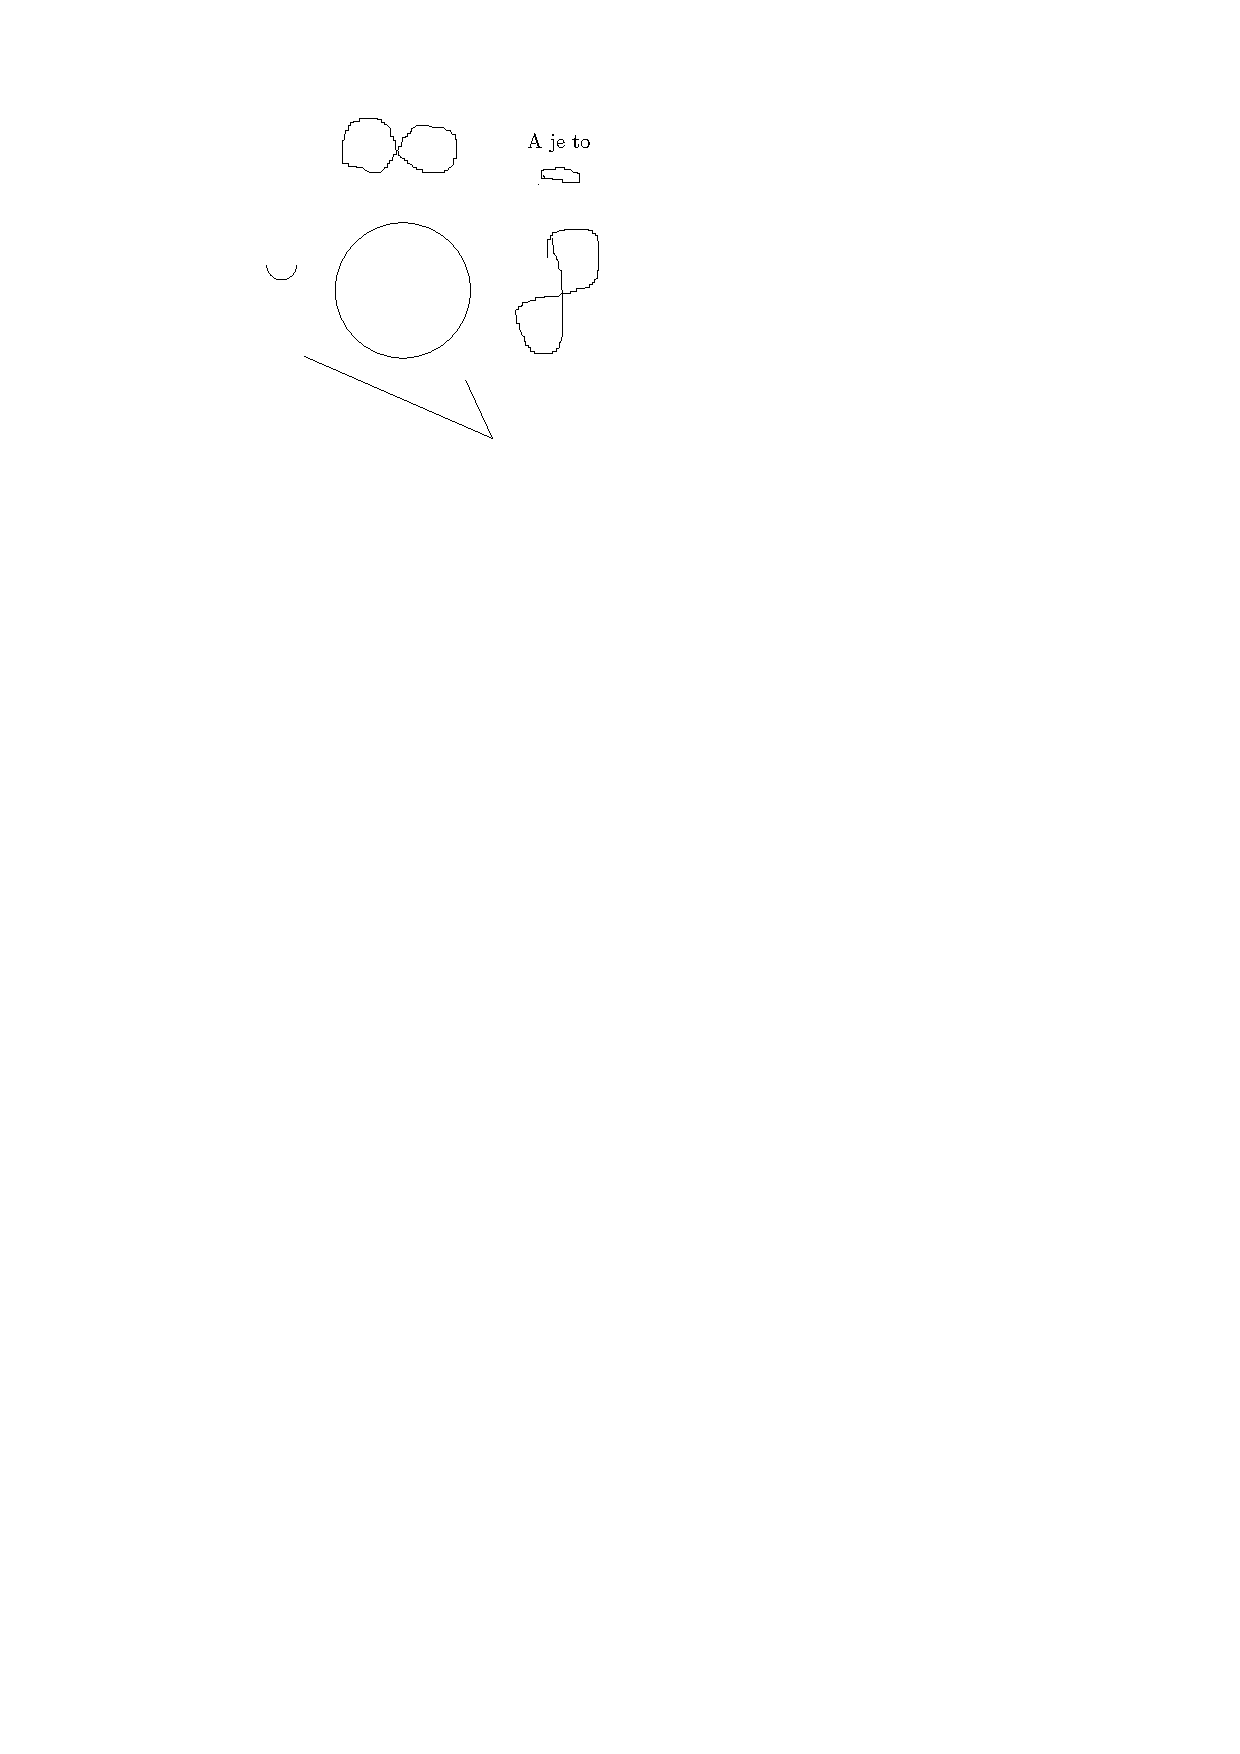
\includegraphics{Obrzkusmo.pdf}
\caption{Obrázek v pdf kreslený v ipe} %popisek obrázku automaticky doplněný o číslo a promítající se v seznamu obrázků
\end{center}
\end{figure}
\vspace*{10mm}
\begin{figure}[h] %obrázek musí být v plovoucím objektu figure; pro zabránění nežádoucího plavání po stránce se musí doplnit parametr "[h]"
\begin{center}
\includegraphics[width=15cm]{58.jpg} %příkaz width zmenší délku na zadaný rozměr fyzického papíru a zachová proporce
\caption{Fotka v jpg} %popisek obrázku automaticky doplněný o číslo a promítající se v seznamu obrázků
\end{center}
\end{figure}


%%Stránka pro zkoušení vkládání tabulek%%
\subsection{Vkládání tabulek}
Zkušební tvorba tabulek. Nejhorší je tvorba sirotků. Otázkou je, jak jím předejít. Klasické parametry nepomáhají. Problém se ani na fórech neřeší\ldots
\begin{table}[h] %tabulka "tabular" musí být uzavřena v plovoucím objektu "table"
\caption{Tabulka s přizpůsobením šířky sloupců}
\begin{center} %pro zarovnání tabulky na střed
\begin{tabular}{|l|c|c|} %zarovnání sloupců |left|center|center| oddělené čárou
\hline %horní horizontální čára
\textbf{Frekvenční pásmo} & \textbf{Technologie} & \textbf{Region} \\ %první řádka
\hline %oddělovací čára
700Mhz & LTE & USA \\ %druhá řádka 
\hline %oddělovací čára
800Mhz & LTE & Evropa \\ %třetí řádka
\hline %oddělovací čára
850Mhz & GSM & USA \\ %čtvrtá řádka
\hline 
900Mhz & GSM & Evropa \\ 
\hline
1700Mhz & 3G & USA \\ 
\hline
1800Mhz & GSM & Evropa \\ 
\hline
1900Mhz & GSM & USA \\ 
\hline 
2100Mhz & 3G & Evropa \\ 
\hline
2600Mhz & LTE & Evropa \\ 
\hline
\end{tabular}
\end{center}
\end{table} 

Fixní šířka sloupce může být nastavena příkazem "p\{5cm\}", ale tento příkaz vynutí zarovnání doleva. Při požadavku na zarovnání na střed nebo doprava ho nelze použít a buňka se musí manuálně roztáhnout doplněním násilných mezer "~" v první řádce tak, aby všechny sloupce byly stejně široké.

\begin{table}[h] %tabulka "tabular" musí být uzavřena v plovoucím objektu "table"
\caption{Tabulka s fixní šířkou sloupců}
%fixní šířka sloupce může být nastavena příkazem "p{5cm}", ale tento příkaz vynutí zarovnání doleva, při požadavku na zarovnání na střed nebo doprava ho nelze použít a buňka se musí manuálně roztáhnout doplněním násilných mezer "~" v první řádce tak, aby všechny sloupce byly stejně široké
\begin{center} %pro zarovnání tabulky na střed
\begin{tabular}{|l|c|c|} %zarovnání sloupců |left|center|center| oddělené čárou
\hline %horní horizontální čára
\textbf{Frekvenční pásmo} & \textbf{~~~Technologie~~~} & \textbf{~~~~~~Region~~~~~~} \\ %první řádka doplněná násilnými mezerami "~" pro rotažení buněk, aby sloupce byly stejně široké
\hline %oddělovací čára
700Mhz & LTE & USA \\ %druhá řádka 
\hline %oddělovací čára
800Mhz & LTE & Evropa \\ %třetí řádka
\hline %oddělovací čára
850Mhz & GSM & USA \\ %čtvrtá řádka
\hline 
900Mhz & GSM & Evropa \\ 
\hline
1700Mhz & 3G & USA \\ 
\hline
1800Mhz & GSM & Evropa \\ 
\hline
1900Mhz & GSM & USA \\ 
\hline 
2100Mhz & 3G & Evropa \\ 
\hline
2600Mhz & LTE & Evropa \\ 
\hline
\end{tabular}
\end{center}
\end{table} 


%%Stránka pro zkušební sazbu rovnic"
\subsection{Sazba rovnic}
Slavná rovnice Alberta Einsteina praví: $E = m \cdot c^2$. Platí pro všechny částice s nenulovou klidovou hmotností. Energie fotonu je naproti tomu determinována pouze jeho frekvencí (a Planckovou konstantou) $E = h * f$.
%sazba rovnice přímo v textu se provádí mezi dvěma znaky "$...$"

Nyní se podíváme na zoubek číslovaným rovnicím. Co třeba takhle první Maxwellova rovnice v diferenciálním tvaru?
\begin{equation} \label{max1} %číslovaná rovnice mimo text se uvádní příkazem "equation"; příkaz "label" slouží pro vytvoření návěští pro hypertextový odkaz na rovnici
\rot\vec{H}=\vec{J}+\dfrac{\partial \vec{D}}{\partial t}
%"\rot" - rotace; "\vec" - znak vektoru; "\frac{•}{•}" - rovnice; "\partial" - znak diferenciální rovnice 
\end{equation}

Pro sazbu matematiky platí obecně jiná pravidla. Jinak se například zadávají mezery nebo tučné písmo.
\begin{equation}
\forall x \in \mathbf{R}: \qquad x^{2+p} \geq 0
%"\forall" - znak "pro všechna"; "\in" - znak "je prvkem"; "\mathbf{•}" - tučné písmo v rovnici; "\qquad" - delší mezera v rovnici; více znaků v jednom místě musí být uzavřeno mezi "{}"; "\geq" - znak "větší nebo rovno"
%pro tučné nevzpřímené symboly je místo "\mathbf{•}" nutno použít "\boldsymbol"
\end{equation}

Zkusíme i odkazování. Vzpomínáte si na první Maxwellovu rovnici? Jestli ne, je to tato: \ref{max1}. Btw., znáte ten hezký symbol pro množinu reálných čísel? Je to tento: $\mathbb{R}$
%"\ref{max1}" - slouží pro vytvoření hypertextového číslovaného odkazu na rovnici (návěští max1)
%"\mathbb{R}" - vloží prokládaný znak R

A teď třeba funkce a odmocniny. Jako příklad do písemky z matematiky. Najděte definiční obor funkce:
\begin{equation}
f(x):\quad\left(\dfrac{\sqrt{3^{-x}}}{\sqrt[3]{x-7}}\right)^2
%"\quad" - mezera; "\left(" - levá závorka přes celou výšku následujícího výrazu (zlomku); "\dfrac" - zlomek; "\sqrt[3]" - 3. odmocnina; "\rigt)" - uzavření závorky přes celou výšku výrazu 
\end{equation} 

Studenti, pamatujete si ještě, derivace? Tohle musíte umět z hlavy i kdybych vás probudil uprostřed noci: $y=\cos(x^3)\qquad y'= \qquad y''=$
%"'" popř. "''" - první popř. druhá derivace

Kdo z vás si vzpomene ještě na limity a ví, co tato znamená?
\begin{displaymath}
\lim_{x \rightarrow 0} \frac{\sin x}{x} = 1
%limita odkud kam se zadává jako dolní index: "lim_{x \rightarrow 0}"; "\rightarrow" - šipka doprava používaná v limitě; "\sin" - sin a další se zadávají přes lomítko, aby byly vzpřímeným písmem
\end{displaymath}

Vrátíme se zpět k Maxwellovým rovnicím. Budeme pokračovat popořadě a podíváme se na druhou Maxwellovu rovnici, tentokrát v integrálním tvaru:
\begin{equation}
\oint_c \vec{E} \overrightarrow{\ud l} = -\frac{\ud\Phi}{\ud t}
%"\oint_c" - křivkový integrál po křivce c (zadává se jako dolní index); "\overrightarrow{•} - šipka vektoru ale přes více znaků; "\ud" - vzpřímené "d" používané v integrálu; "\Phi" - velké řecké fí 
\end{equation}

A nyní něco trochu komplikovanějšího. Jak se spočte taková zřídlovost?
\begin{equation}
\nabla \times \vec{E} = \rot \vec{E} = \left| 
%"\nabla" - nabla; "\times" - vektorové "krát"; "\rot" - rotace; "\left|" - závorky determinantu
\begin{array}{c c c}
%determinant nebo matice se zadávají přes prostředí "array", parametry udávají počet sloupců a jejich centrování ("c" - na střed)
\vec{i} & \vec{j} & \vec{k} \\
%zadávání jako u tabulky: "&" pro další buňku, "\\" pro další řádek
\frac{\partial}{\partial x} & \frac{\partial}{\partial y} & \frac{\partial}{\partial z} \\
E_x & E_y & E_z
\end{array} \right|
\end{equation}

Občas bude zapotřebí vysázet víc rovnic současně. Například všechny Maxwellovy rovnice. Následující ukázka předvádí použití příkazu "eqnarray" nahrazující "equation" pro sazbu více rovnic. Rovnítko se musí doplnit znaky "\&": "\&=\&", aby byly rovnice správně vycentrovány na střed.
\begin{eqnarray}
%prostředí "eqnarray" nahrazuje "equation" pro sazbu více rovnic
f(x)&=&\cos x
%rovnítko se musí doplnit znaky "\&": "\&=\&", aby byly rovnice správně vycentrovány na střed
\\
f'(x)&=&-\sin x
\\
\udiv x &=& 0
%pro divergenci se musí použít "\udiv" namísto "\div"
\end{eqnarray}

\noindent
%"\noindent" - zajistí, že následující odstavec na začátku nebude odsazený
Nebo napsat vysvětlivku k rovnici, která nebude odsazená.


%Zkušební stránka odrážek a číslování%%
\subsection{Odrážky a číslování}

\subsubsection{Odrážkovaný seznam}
Státy USA, které jsem navštívil:
\begin{itemize}
%prostředí "itemize" vytvoří zařážkový seznam; příkaz "\item[-]" může být doplněn "-" pro nahrazení koleček pomlčkami
\item Kalifornie
%příkazem "\item" se přidávají jednotlivé položky
\item Florida
\item New Jersey
\item New York
\item Illinois
\item Wisconsin
\item Minnesota
\item Pensylvánie
\item Maryland
\item Virginia
\item District of Columbia
\end{itemize}

\subsubsection{Číslovaný seznam}
Pořadí, v jakém jsem je navštívil:
\begin{enumerate}
%prostředí "enumerate" vytvoří číslovaný seznam
\item Illinois
%příkazem "\item" se přidávají jednotlivé položky
\item Wisconsin
\item Minnesota
\item Kalifornie
\item New York
\item New Jersey
\item Pensylvánie
\item Maryland
\item District of Columbia
\item Virginia
\item Florida
\end{enumerate}

\subsubsection{Popisné výčty (prostředí ,,Description'')}
Hlavní města některých států USA, které jsem navštívil:
\begin{description}
%prostředí description vytvoří seznam, kde je první část (název) zvýrazněno, za ním následuje text
\item[Kalifornie] Sacramento
%příkazem "\item[]" se přidávají jednotlivé položky, do "[]" se uvede název (to co bude tučně)
\item[Wisconsin] Madison
\item[Maryland] Annapolis
\end{description}

\subsubsection{Odsazování - tabulátor}
Největší města některých států USA, která jsem navštívil:
\begin{tabbing} %začátek odsazovaného prostředí tabulátoru
\hspace{5cm}\=\kill %parametrem v "\hspace{•cm}" je délka odsazení tabulátoru
Illinois \> Chicago \\ %nejdříve první část, potom tabulátor "\>" a druhá část
Maryland \> Baltimore \\ 
Kalifornie \> Los Angeles 
\end{tabbing} 

\subsection{Citace}
\LaTeX ~nabízí i speciální prostředí pro citace a zvýraznění textu:
\begin{quote} %začátek prostředí pro citaci
\emph{,,Veni, vidi, vici.''} %zvýraznění (kurzíva) citace 
\end{quote}

\subsection{Verbatim}
Prostředí ,,Verbatim'' se hodí na sazbu textů, kde není žádoucí brát zřetel na formátovací značky. Příkladem je sazba zdrojových kodů.
%začátek prostředí verbatim pro sazbu bez ohledu na formátovací značky
\begin{verbatim}
System.out.println("Ja su lama, nevzpomenu si ani na zapis hlavicky v Jave")
\end{verbatim}


%%Závěr%%
\clearpage %\newpage nefunguje, po plouvocím objektu (obrázek, tabulka) musí pro novou stránku následovat "clearpage" 
\section{Závěr}
Modleme se za to, že se práce úspěšně povede dotáhnout do konce a v dubnu tady bude moci čnít: ,,Práce dokončena''

In nomine Patris et Filii et Spiritus Sancti. Amen.

%%Použitá literatura%%
\newpage
\phantomsection %Pro správné zobrazení čísla stránky v pdf rejsříku a přesný hyperodkaz
\addcontentsline{toc}{section}{Použitá literatura}
\begin{thebibliography}{10}

%Do "{}" příjmení autora, za to vložit z citace.cz, na název kurzívu
%Podle názvu v "{}" se poté odkazuje uvnitř textu pomocí příkazu "\cite{}" 
\bibitem{Pozar} POZAR, David M. \textit{Microwave Engineering}. John Wiley \& Sons, Inc., 1998. Second Edition. ISBN 0-471-17096-8.

\end{thebibliography}

%%Seznam obrázků%%
\newpage
\phantomsection %Pro správné zobrazení čísla stránky v pdf rejsříku a přesný hyperodkaz
\addcontentsline{toc}{section}{Seznam obrázků}
\setlength{\parskip}{0ex}%Aby nebyly moc velké mezery mezi řádky seznamu obrázků a tabulek
\listoffigures

%%Seznam tabulek%%
\newpage
\phantomsection %Pro správné zobrazení čísla stránky v pdf rejsříku a přesný hyperodkaz
\addcontentsline{toc}{section}{Seznam tabulek}
\listoftables

%%Přílohy%%
\newpage
\pagestyle{empty} %vypnutí číslování
\setcounter{page}{1} %číslo stránky nastaveno na "1"
\appendix %deklarace, že se jedná o přílohu
\phantomsection %Pro správné zobrazení čísla stránky v pdf rejsříku a přesný hyperodkaz
\addcontentsline{toc}{section}{Přílohy}
\section*{Příloha I.}

\end{document}
